\chapter{Solution}
\minitoc

The main goal of this solution is to develop a recommendation system for an e-commerce platform. 
In this context, users are referred to as customers or buyers ( representing individuals interacting with the platform which can be through a website or an app ), 
while products are referred to as items ( representing the goods offered for sale ).

To operate all the stages of the recommendation pipeline and the system components, 
a lot of infrastructure and DevOps work is required, from data ingestion to the deployment of the components, Figure~\ref{fig: SystemComponents} shows a suggested system design by Nvidia.

The following sections will explain the system components and the deployment and technologies used in each stage of the recommendation pipeline.

The system components can be divided into the following categories:
\begin{itemize}
    \item API gateway
    \item Storage Components
    \item Recommendation Pipeline (Offline)
    \item Inference Ensemble (Online)
    \item Caching Layer
    \item Automation and DevOps
\end{itemize}

\begin{figure}[H]
    \centering
    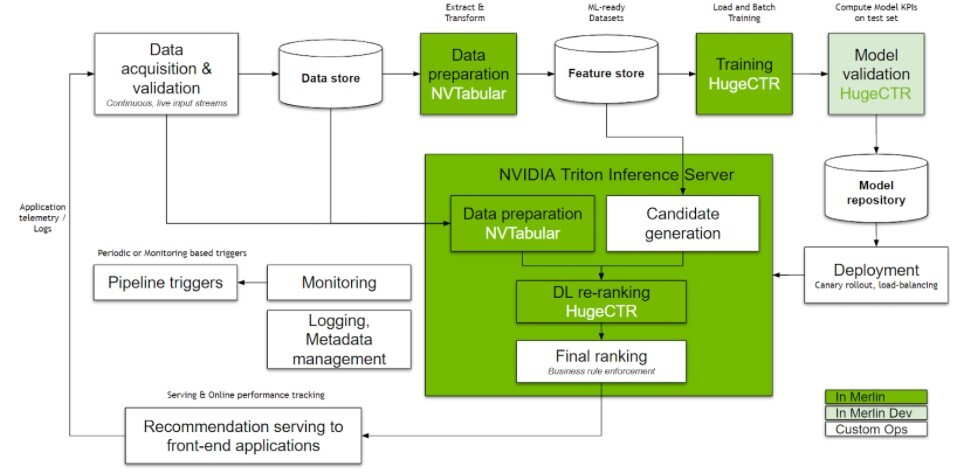
\includegraphics[width=\textwidth]{assets/components.jpeg}
    \caption[System Components]{System Components~\cite{NvidiaRecSysBestPractices}}
    \label{fig: SystemComponents}
\end{figure}

Each component is explained in the following sections.

\section{API Gateway}

The API gateway, a RESTful API, is the entry point for the recommendation system.
It is responsible for handling all the requests and responses from the customers.
The main two functionalities of the API gateway are data ingestion and getting recommendations for a customer.

In addition to these functionalities, the API gateway is also responsible for authenticating and authorizing the requests.

\subsection{Data Ingestion Endpoints}

To handle the data ingestion, the API gateway exposes the following endpoints:
\begin{itemize}
    \item CRUD customers
    \item CRUD products
    \item Adding interactions between customers and products
\end{itemize}

Such endpoints interact mainly with the storage components to store the data.

\subsection{Recommendation Endpoints}

To get recommendations for a customer, the API gateway exposes the following endpoint:
\begin{itemize}
    \item Get recommendations for a customer
    \item Get similar products to a product
\end{itemize}

Those endpoints interact mainly with the recommendation pipeline and the caching layer to get the recommendations.

The first endpoint queries the caching layer to get the recommendations, and if the offline recommendations are not found in the caching layer, 
the API gateway queries the recommendation pipeline to get online recommendations, and then stores the recommendations in the caching layer, 
after getting the recommendations from the recommendation pipeline, 
the API gateway orders the recommendations using the output of the ranking stage and using business rules, then returns the top recommendations to the customer.

In the second endpoint, the API gateway queries a different ensemble that uses the item embedding as a query instead of the user embedding.

\section{Storage Components}

The storage components are responsible for storing the data in different formats and stages, in addition to the models used in the recommendation system.
There are four main storage components in the system:

\begin{itemize}
    \item Main Database
    \begin{displayquote}
        The main database is an SQL database that stores the customers, products, and
         interactions data. In this project, a PostgreSQL~\cite{Postgres} instance 
         deployed using AWS RDS \footnote{AWS Relational Database Service~\cite{AwsRDS}}
         is used as the main database. 
         But in a bigger production environment, a distributed Data Warehouse such as 
         Amazon Redshift~\cite{AwsRedshift} or Google BigQuery~\cite{GoogleBigQuery} can be used.
    \end{displayquote}
    \item Online Feature Store
    \begin{displayquote}
        The feature store is a storage system that stores data in a format optimized for ML models.~\cite{NvidiaFeatureStores}
        It also stores the embedding tables of the customers 
        and products, in addition to any other categorical features.
        This project uses FEAST~\cite{feast} as the feature store, which supports using a Redis~\cite{Redis} 
        cluster as an Online store, the Redis cluster is deployed using AWS ElastiCache~\cite{AwsElastiCache}.
    \end{displayquote}

    \item Item Embedding Store
    \begin{displayquote}
        A vector database that stores the embeddings of the products
        while allowing them to be queried using an ANN search algorithm. 
        In this project, the item embedding store is a Faiss Index\cite{Faiss} that is stored in an S3 bucket and is materialized, loaded in memory, on inference server startup.
    \end{displayquote}

    \item Model Repository
    \begin{displayquote}
        After training the models, their parameters are stored in the model repository. In this project, the model repository is an AWS S3 bucket~\cite{AwsS3}. 
    \end{displayquote}
    \item Results Store
    \begin{displayquote}
       To implement offline batch recommendations, the results of running the recommendation pipeline periodically for all users are stored in the results store. 
       In this project, the results store is a Redis\cite{Redis} cluster deployed using AWS ElastiCache~\cite{AwsElastiCache}.
    \end{displayquote}
\end{itemize}

